\renewcommand{\theequation}{\theenumi}
\begin{enumerate}[label=\thesection.\arabic*.,ref=\thesection.\theenumi]
\numberwithin{equation}{enumi}
\item 
\label{ex:ellipse_tangent}
Find $\frac{dy}{dx}$ if 
%\cite{twelve_one}
\begin{align}
E_1: x^2 + xy +y^2  = 100
\label{eq:ellipse}
\end{align}
\solution Expressing \eqref{eq:ellipse}  as \eqref{eq:conic_quad_form}, 
\begin{align}
\vec{V} = \myvec{1 & \frac{1}{2} \\ \frac{1}{2} & 1}, \vec{u} = \vec{0}, f = -100.
\label{eq:ellipse_ips}
\end{align}
%
\begin{align}
\because \abs{V} = \mydet{1 & \frac{1}{2} \\ \frac{1}{2} & 1} > 0,
\end{align}
\eqref{eq:ellipse} is the equation of an ellipse. To verify that this is indeed the case, we do the following exercise.
%
The characteristic equation of $\vec{V}$ is obtained by evaluating the determinant
\begin{align}
\mydet{\lambda \vec{I}-\vec{V}} = \mydet{\lambda -1 & \frac{1}{2}\\ \frac{1}{2} & \lambda -1} &= 0
\\
\implies \lambda^2 - 2\lambda + \frac{3}{4} &= 0
\label{eq:ellipse_char}
\end{align}
The eigenvalues are the roots of \eqref{eq:ellipse_char} given by
\begin{align}
\lambda_1 = \frac{1}{2}, \lambda_2 = \frac{3}{2}
\label{eq:ellipse_eval}
\end{align}
The eigenvector $\vec{p}$ is defined as
\begin{align}
\vec{V} \vec{p}&= \lambda \vec{p}
\\
\implies \brak{\lambda\vec{I}-\vec{V}}\vec{p} &=0
\end{align}
where $\lambda$ is the eigenvalue.  For $\lambda_1 = \frac{3}{2}$,
\begin{align}
\brak{\lambda_1\vec{I}-\vec{V}}
= \myvec{\frac{1}{2} & -\frac{1}{2}
\\ -\frac{1}{2} & \frac{1}{2}} 
\xleftrightarrow[R_1 \leftarrow 2R_1] {R_2\leftarrow R_2-R_1}\myvec{1 & -1 \\0 & 0 }  
\\
\implies \vec{p}_1 = \frac{1}{\sqrt{2}}\myvec{1 \\ 1}
\end{align}
such that $\norm{\vec{p}_1} = 1$.  Similarly, the eigenvector corresponding to $\lambda_2$ can be obtained as
\begin{align}
 \vec{p}_2 = \frac{1}{\sqrt{2}}\myvec{-1 \\ 1}
\end{align}
It is easy to verify that 
\begin{align}
\label{eq:ellipse_spectrum}
%\begin{split}
%\myvec{1 & \frac{1}{2}\\ \frac{1}{2} & 1} &= \frac{1}{\sqrt{2}}\myvec{1 & 1\\ 1 & -1}\myvec{\frac{3}{2} & 0\\ 0 & \frac{1}{2}}\frac{1}{\sqrt{2}}\myvec{1 & 1\\ 1 & -1}
%\\
%\text{or, }
\vec{V} &= \vec{P}\vec{D}\vec{P}^{-1}=\vec{P}\vec{D}\vec{P}^T \quad \because \vec{P}^{-1} = \vec{P}^{T}
\\
\text{or, } \vec{D} &= \vec{P}^T\vec{V}\vec{P}
%\end{split}
\end{align}
where 
\begin{align}
\label{eq:ellipse_spectrum_P}
\vec{P} & =\myvec{\vec{p}_1 & \vec{p}_2} = \frac{1}{\sqrt{2}}\myvec{1 & 1\\ -1 & 1}
\\
 \vec{D} &= \myvec{\lambda_1 & 0 \\ 0 & \lambda_2} =\myvec{\frac{3}{2} & 0\\ 0 & \frac{1}{2}}
\label{eq:ellipse_spectrum_D}
\end{align}
From Table \ref{table:conics}, ellipse parameters are given by
\begin{align}
\vec{c} =-\vec{V}^{-1}\vec{u} &= \vec{0}
\\
\sqrt{\frac{\vec{u}^T\vec{V}^{-1}\vec{u}-f}{\lambda_1}} &= 10 \sqrt{\frac{2}{3}}
\\
\sqrt{\frac{\vec{u}^T\vec{V}^{-1}\vec{u}-f}{\lambda_2}} &= 10 \sqrt{2}
\end{align}
In Fig. \ref{fig:ellipse_tangent} the actual ellipse ellipse in \eqref{eq:ellipse} is obtained from \eqref{eq:conic_simp_temp_nonparab} using \eqref{eq:conic_affine}.  The anticlockwise 45\degree rotation is due to the fact that 
\eqref{eq:ellipse_spectrum_P} can be expressed as
\begin{align}
\label{eq:ellipse_spectrum_P_rot}
\vec{P}  = \myvec{\cos 45\degree & -\sin 45\degree\\ \sin 45\degree & \cos 45\degree}
\end{align}
Coming back to the original question of finding $\frac{dy}{dx}$,
if the point of contact
\begin{align}
\vec{q} = \myvec{q_1\\q_2},
\end{align}
from \eqref{eq:ellipse_ips},
\eqref{eq:dir_vec_slope}
and \eqref{eq:conic_tangent_mq},
%
\begin{align}
\myvec{1 & m}\myvec{1 & \frac{1}{2} \\ \frac{1}{2} & 1}\myvec{q_1\\q_2} &= 0
\\
\implies \myvec{1 + \frac{m}{2} & \frac{1}{2}+m}\myvec{q_1\\q_2} &=0
\\
\implies \frac{m}{2} \brak{q_1+2q_2} + q_1 + \frac{q_2}{2} &= 0
\\
\text{or, } m = \frac{dy}{dx}= -\frac{2q_1+q_2}{q_1+2q_2}
\label{eq:conic_tangent_slope}
\end{align}
$\because \frac{dy}{dx}$ is the slope of the tangent.
Note that no results from differential calculus were used to obtain \eqref{eq:conic_tangent_slope}.

\begin{figure}[!ht]
\centering
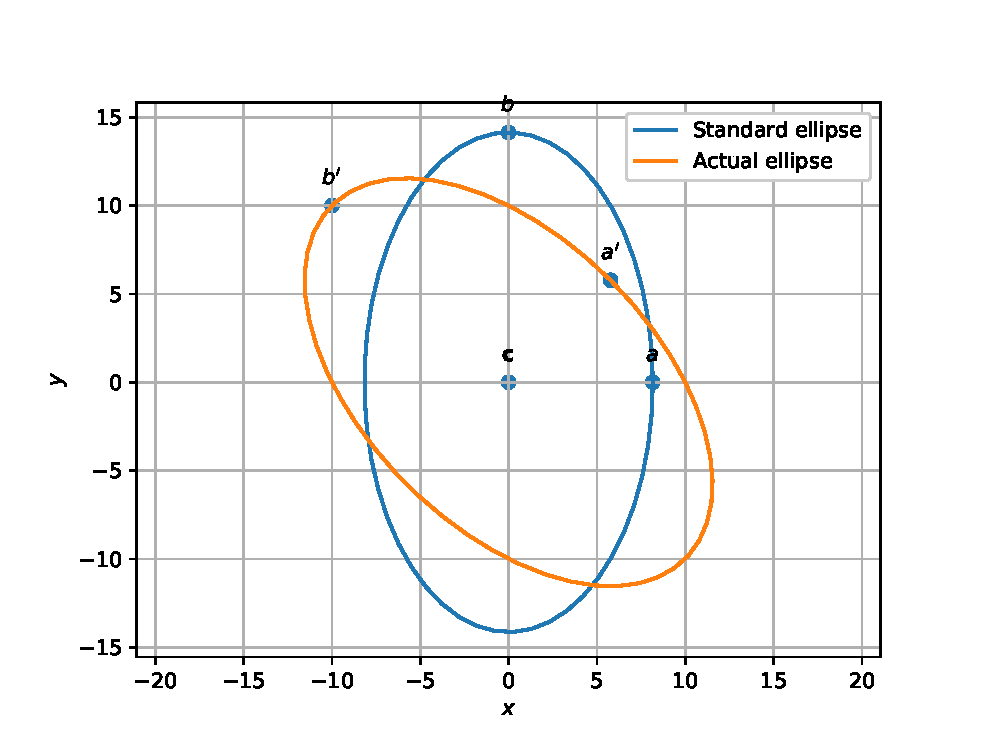
\includegraphics[width=\columnwidth]{./figs/ellipse/ellipse_tangent.eps}
\caption{Actual ellipse and transformed ellipse.}
\label{fig:ellipse_tangent}	
\end{figure}
%
\item 
Find the equation of the ellipse, with major axis along the x-axis and passing through the points $\vec{a} = \myvec{4\\3}$  and $\vec{b} = \myvec{– 1\\4}$ 
%\cite{eleven}.
\\
\solution This is a standard ellipse given by 
\begin{align}
\label{eq:ellipse_std}
\vec{x}^T\vec{D}\vec{x} = 1, \quad \vec{D} = \myvec{\lambda_1 & 0 \\ 0 & \lambda_2}, \lambda_1,\lambda_2 > 0
\end{align}
$\because \vec{a}, \vec{b}$ satisfy \eqref{eq:ellipse_std},
\begin{align}
\label{eq:ellipse_std_ab}
\vec{a}^T\vec{D}\vec{a} &= 1,
\\
\vec{b}^T\vec{D}\vec{b} &= 1
\end{align}
%
which can be expressed as
\begin{align}
\label{eq:ellipse_std_ab_diag}
\begin{split}
\vec{a}^T\vec{A}\vec{d} &= 1,
\\
\vec{b}^T\vec{B}\vec{d} &= 1
\end{split}
\end{align}
%
where
\begin{align}
\vec{d} = \myvec{\lambda_1\\ \lambda_2},
\vec{A} = \myvec{4 & 0 \\ 0 & 3},
\vec{B} = \myvec{-1 & 0 \\ 0 & 4}.
\end{align}
\eqref{eq:ellipse_std_ab_diag}
can then be expressed as the matrix equation
\begin{align}
\label{eq:ellipse_std_ab_diag_mateq}
\myvec{\vec{a}^T\vec{A}\\ \vec{b}^T\vec{B}}\vec{d} &= \myvec{1\\1},
\end{align}
which, after substituing the appropriate values can be expressed as
\begin{align}
\label{eq:ellipse_std_ab_diag_mateq_subs}
\myvec{16 & 9\\ 1 & 16}\vec{d} &= \myvec{1\\1},
\end{align}
Forming the augmented matrix and performing row reduction,
\begin{align}
\myvec{16 & 9 & 1\\ 1 & 16 & 1} 
\xleftrightarrow[R_2\leftarrow -R_2]{R_2\leftarrow R_1}
\myvec{1 & 16 & 1 \\ 0 & 247 & 15} 
\\
\xleftrightarrow[]{R_1\leftarrow 247R_1-16R_2}
\myvec{247 & 0 & 7 \\ 0 & 247 & 15} 
\\
\implies \vec{d} = \frac{1}{247}\myvec{7\\15}, \text{ or, } \vec{D} = \frac{1}{247}\myvec{7 & 0 \\ 0 & 15}
\end{align}
The ellipse parameters are obtained from Table \ref{table:conics} as
\begin{align}
\vec{c} = \vec{0},
\frac{1}{\sqrt{\lambda_1}}  = \sqrt{\frac{247}{7}},
\frac{1}{\sqrt{\lambda_2}}  = \sqrt{\frac{247}{15}}.
\end{align}

Fig. \ref{fig:ellipse_secant}	verifies the above results.
\begin{figure}[!ht]
\centering
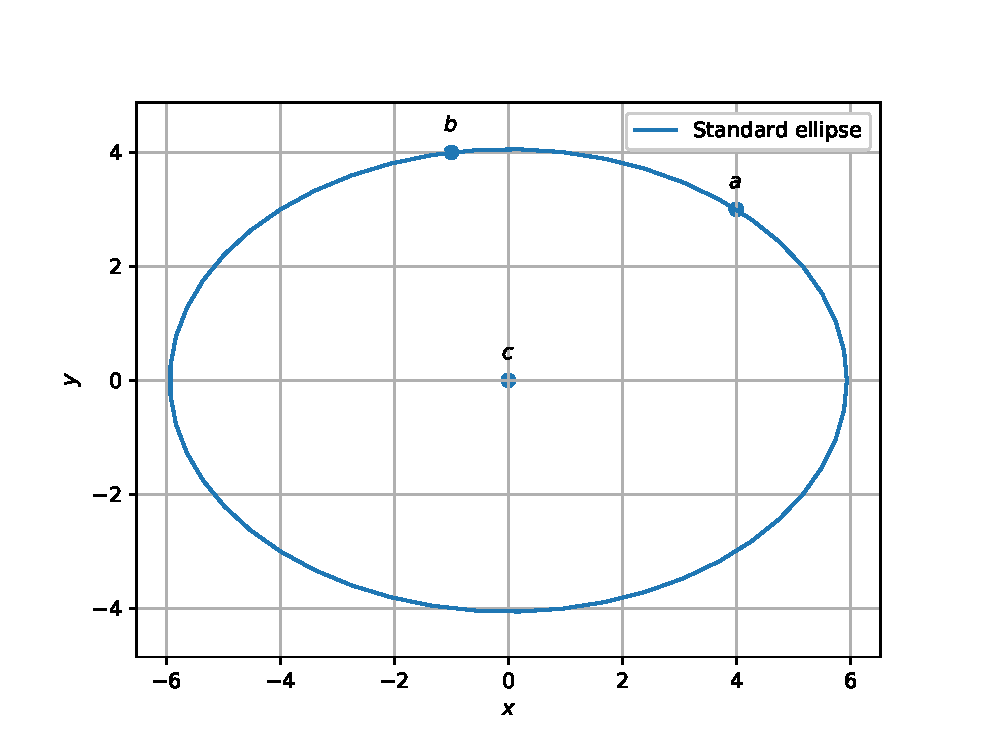
\includegraphics[width=\columnwidth]{./figs/ellipse/ellipse_secant.eps}
\caption{Ellipse through the given points $\vec{a} = \myvec{4\\3}$  and $\vec{b} = \myvec{– 1\\4}$.}
\label{fig:ellipse_secant}	
\end{figure}


\end{enumerate}
